\documentclass[../main/main.tex]{subfiles}

\newdate{date}{14}{10}{2020}


\begin{document}

Una volta scelti i valori di resistenze per costruire il ponte di Wheatstone, abbiamo utilizzato il lock-in per ridurre il rumore ed effettuare una calibrazione precisa in AC.
Infatti, aumentando il guadagno del lock-in riusciamo ad ottenere una calibrazione sempre più precisa. Purtroppo, si raggiunge un punto in cui la sensibilità della manopola del potenziometro sarà non sufficiente per calibrare il circuito. Quindi il guadagno non può essere aumentato troppo ma solo fino al punto in cui girando di non troppo la manopola si vedono delle leggere variazioni. Quando praticamente sfiorando la manopola si vedono grandi variazioni significa che abbiamo impostato un guadagno troppo alto.
\marginpar{ \textbf{Laboratory 3.} \\  \displaydate{date}. \\ Compiled:  \today.}

Domanda: perché il lock-in riduce il rumore e ci permette di fare una calibrazione precisa?
Il lock-in riduce il rumore perchè genera onde in un range di 30 Hz e poi integra il segnale in quel range \( \pm \) 0.1 (dove questo valore è dato dal valore della costante di tempo che è inversamente proporzionale alla lunghezza della banda passante). Invece l'oscilloscopio integra su una banda molto grande, fino al range dei MHz. Questo fa si che utilizzare il lock-in sia molto conveniente. Inoltre ci fa capire perchè i circuiti in AC siano preferibili rispetto a quelli in DC. Infatti, con un circuito in DC non avremmo potuto fare la stessa cosa perché non avevamo un onda portante ad una data frequenza.

Oggi abbiamo calibrato il circuito (ponendo a zero in AC la differenza di potenziale \( V_{AB} \)) impostando un guadagno del lock-in di \( \sim \times  4.85 \).

\begin{remind}{Configurazione ponte e calibrazione AC finale}{}
    Prima di passare alla sezione successiva in cui dovremo costruire l'amplificatore differenziale, facciamo un recap della disposizione di questo circuito prima di smontarlo. Per la volta prossima è importante ricordare che:
    \begin{itemize}
    \item il circuito finale è organizzato come in Fig. \ref{fig:3_2}.
    \item in particolare, i connettori banana rossi e verdi sono collegati al trasformatore dal quale viene preso il segnale in ingresso. Questi cavi banana sono connessi sul retro del trasformatore come in Fig. \ref{fig:3_1}.
    \item il connettore banana-bnc (bianco e rosso) serve per misurare la tensione ai capi delle resistenze \( R_1 \) e \( R_2 \) per regolare la differenza di tensione \( V_{AB} \) a zero. Per fare ciò viene collegato al lock-in per fare la calibrazione. Per connetterlo al lock-in, collegare la parte bnc sul retro del trasformatore come alla sinistra di Fig. \ref{fig:3_1}. E' importante notare che la leva deve essere impostata su EXT.
    \end{itemize}
\end{remind}


\begin{figure}[h!]
\centering
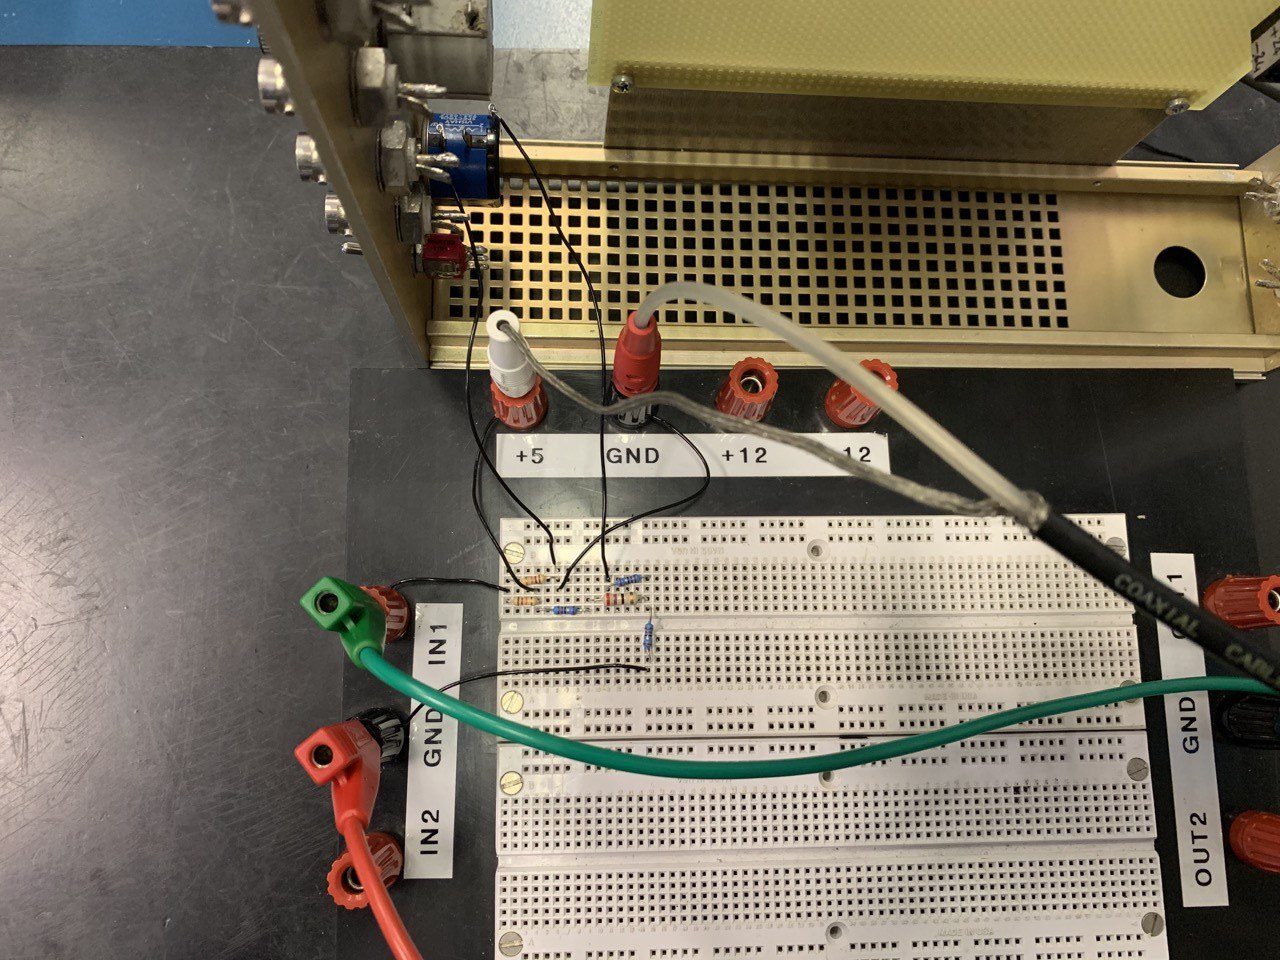
\includegraphics[width=0.8\textwidth]{../lessons/image/03/2.png}
\caption{\label{fig:3_2} Circuito finale del termometro calibrato in AC.}
\end{figure}

\begin{figure}[h!]
\centering
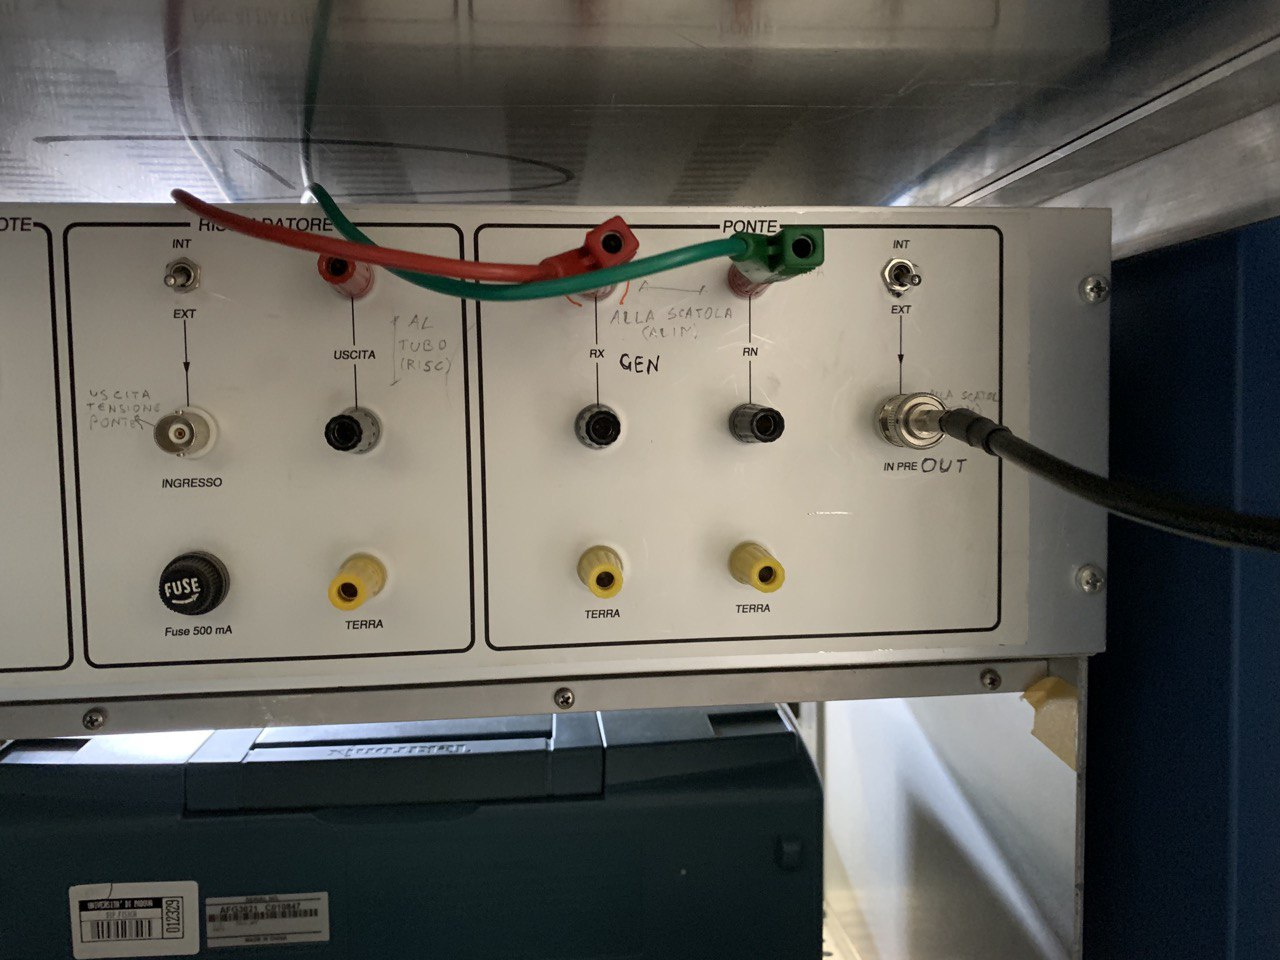
\includegraphics[width=0.8\textwidth]{../lessons/image/03/1.png}
\caption{\label{fig:3_1} Segnale in ingresso dal trasformatore, come inserire i cavi banana e dove.}
\end{figure}


\chapter{Costruzione dell'amplificatore differenziale}

\section{Amplificatore differenziale}
Adesso andiamo a costruire il circuito per realizzare l'amplificatore differenziale che verrà connesso ai capi del nostro superconduttore di cui vogliamo misurare la tensione. Infatti il superconduttore avrà una resistenza molto piccola (parliamo dell'ordine di 0.1 \( \Omega  \)), quindi per misurarla dobbiamo amplificare il segnale di tensione ai capi di questa. Per questo utilizziamo l'amplificatore INA114AP che verrà collegato al materiale che andremo a misurare attraverso i 4 terminali in argento che questo presenta.

L'amplificatore INA114AP è particolare in quanto è un insieme di tanti amplificatori. Come un normale amplificatore, dobbiamo dargli un'alimentazione in ingresso \( V_+ \) e \( V_- \). Bisogna fare attenzione in questa parte qua. Infatti, consideriamo la tensione in uscita dall'amplificatore \( V_0 \), questa non può essere più grande del segnale che alimenta il nostro circuito che sarà di \( \pm 12 \) V. Questo problema può sorgere se per esempio abbiamo una tensione ai capi del superconduttore che è di circa 0.1 V e noi vogliamo amplificarla con un guadagno \( \times 500 \). In questo caso otteniamo \( V_0 \sim 50 \) V. Abbiamo raggiunto la saturazione.


\begin{figure}[h!]
\centering
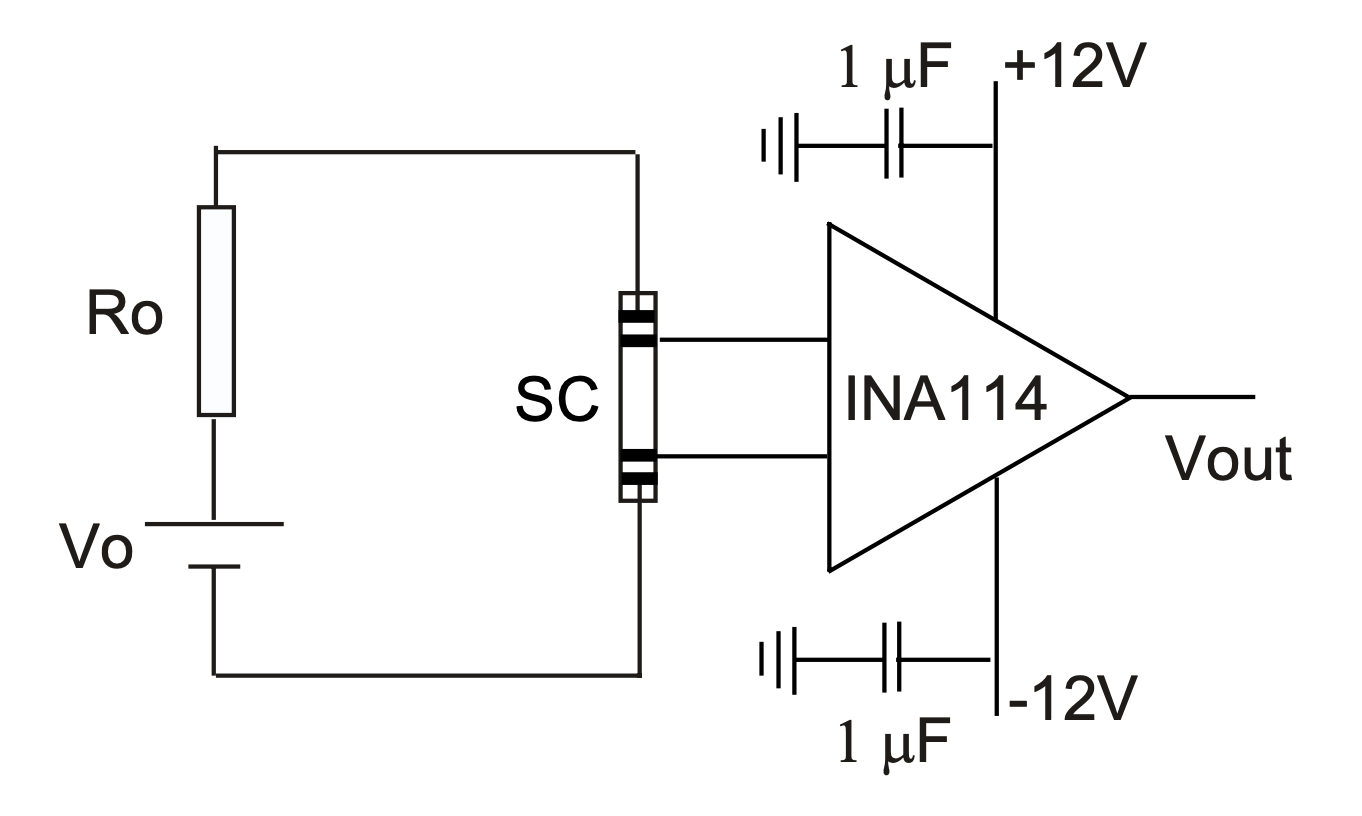
\includegraphics[width=0.6\textwidth]{../lessons/image/03/5.png}
\caption{\label{fig:3_5} Circuito amplificatore differenziale.}
\end{figure}

Il nostro obbiettivo è  montare il circuito in Fig. \ref{fig:3_5} e chiamiamo la resistenza e la tensione ai capi del superconduttore \( R_{sc} \) e \( V_{sc} \).
Adesso l'idea è che dobbiamo alimentare il nostro circuito con una \( V_0 \) che deve essere continua e per fare ciò bisogna prendere una  \( R_0 \) molto grande in modo tale che valga approssimativamente la seguente formula:
\begin{equation*}
 V_{sc} = V_0 \frac{R_{sc}}{R_{sc}+R_0} \sim V_{sc} = R_{sc} I \quad \text{ dove } I = \frac{V_0}{R_0}
\end{equation*}
cioè che la tensione calcolata dalla formula del partitore di tensione sia approssimativamente uguale a un calcolo fatto come se la corrente fosse costante e quindi abbiamo un generatore di tensione continuo.
Questo può valere se prendiamo una \( R_0 \) sufficientemente grande perchè invece la resistenza del superconduttore sarà piccola e trascurabile (\( \sim 0.1 \Omega \)). In questo modo otteniamo anche una tensione piccola ai capi del conduttore, che però andrà amplificata.

\begin{example}{Circuito di prova per far funzionare l'amplificatore}{}
Per prima cosa vogliamo far funzionare l'amplificatore. I valori scelti per \( R_0 \) e \( V_0 \) non saranno uguali a quelli che poi dovremmo scegliere quando utilizzeremo effettivamente il superconduttore, ma servono per ricreare una differenza di potenziale \( V_{sc} \) simile a quella che poi avremo in quel caso.

Se scegliamo:
\begin{itemize}
\item \( V_0 = 1 \) V
\item \( R_{sc} = 10 \Omega \)
\item \( R_0 = 2.5 \text{k} \Omega  \)
\end{itemize}
Otteniamo che:
\begin{equation*}
  I = \frac{V_0}{R_0} = 0.4 \, \text{mA} \quad \Rightarrow \quad V_{sc} = R_{sc} I = 4 \,\text{mV}
\end{equation*}
Vediamo se questo risultato è consistente facendo i calcoli più complessi con il partitore di tensione:
\begin{equation*}
  V_{sc} = V_0 \frac{R_{sc}}{R_{sc}+R_0} = 3.98406 \, \text{mV}
\end{equation*}
I risultati sono consistenti.
Se inoltre impostiamo un guadagno \( G = 100 \), otteniamo:
\begin{equation*}
  V_{out} \equiv V_0 = G(V_{IN}^+ - V_{IN}^-) = 100 \times 4 \,\text{mV} = 400 \,\text{mV}
\end{equation*}
\end{example}

\begin{example}{Circuito per il superconduttore}{}
Adesso vogliamo realizzare il circuito al quale verrà collegato il superconduttore e vogliamo ottenere una differenza di potenziale \( V_{sc} \) simile a quella di prima. Se abbiamo:
\begin{itemize}
\item \( V_0 = 1 \) V
\item \( R_{sc} = 0.1\, \Omega \)
\item \( V_{sc} = 4 \,\text{mV}  \)
\end{itemize}
dobbiamo avere una \( R_0 \) di:
\begin{equation*}
   V_{sc} = V_0 \frac{R_{sc}}{R_{sc}+R_0} \rightarrow R_0 = R_{sc} \qty(\frac{V_0}{V_{sc}} -1) = 24.9 \, \Omega
\end{equation*}
E' troppo piccola, non soddisfa la condizione di corrente continua!
Dobbiamo cambiare strategia. Scegliamo:
\begin{itemize}
\item \( V_0 = 5 \) V
\item \( R_{sc} = 0.1 \, \Omega \)
\item \( V_{sc} = 0.4 \,\text{mV}  \)
\end{itemize}
\begin{equation*}
  V_{sc} (R_{sc} + R_0) = V_0 R_{sc} \rightarrow R_0 = R_{sc} \qty(\frac{V_0}{V_{sc}} -1) = 1.249 \, \text{k}\Omega
\end{equation*}
Se inoltre impostiamo un guadagno \( G = 500 \), otteniamo:
\begin{equation*}
  V_{out} \equiv V_0 = G(V_{IN}^+ - V_{IN}^-) = 500 \times 0.4 \,\text{mV} = 200 \,\text{mV}
\end{equation*}
Ricordare bene che un guadagno alto dell'amplificatore può causare oscillazioni, quindi non esagerare.
\end{example}

Lo schema dell'amplificatore utilizzato è illustrato in Fig. \ref{fig:3_3}. In particolare, facciamo attenzione alla resistenza \( R_G \) che dobbiamo inserire per scegliere il guadagno che vogliamo ottenere come:
\begin{equation*}
  G = 1 + \frac{50 \text{k} \Omega}{R_G}
\end{equation*}
Il pinnaggio dell'amplificatore è illustrato in Fig. \ref{fig:3_4}. I pin di nostro interesse sono \( V_{IN}^- \) e \( V_{IN}^+ \) (terminali ingresso dal superconduttore), \( V_- \) e \( V_+ \) che sono i terminali di alimentazione (\( \pm \) 12 V), e infine ci interessa il pin \( V_0 \) dal quale vediamo l'uscita:
\begin{equation*}
  V_{out} = V_0 = G(V_{IN}^+ - V_{IN}^-)
\end{equation*}

\begin{figure}[h!]
\centering
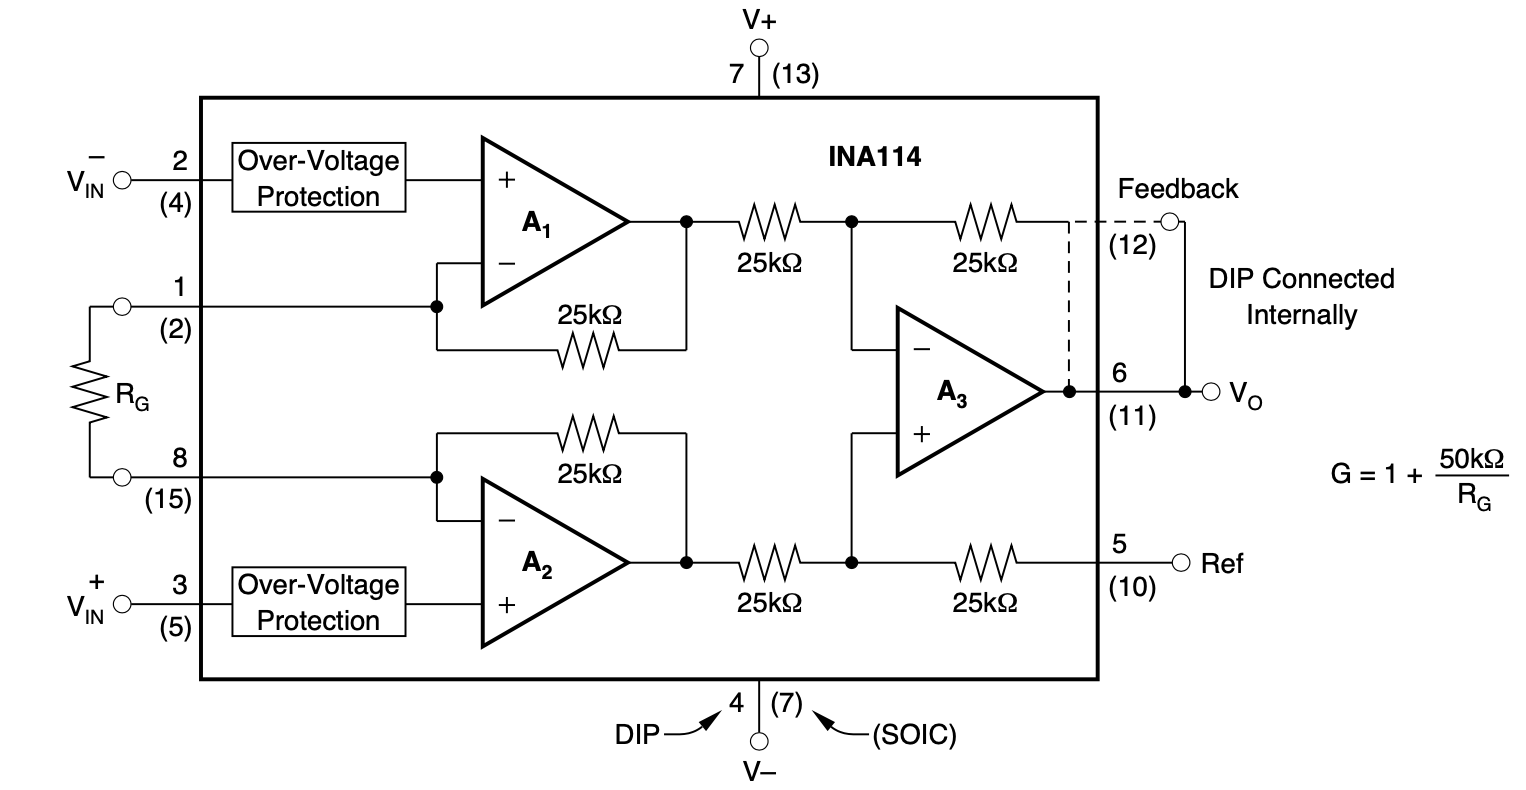
\includegraphics[width=0.6\textwidth]{../lessons/image/03/3.png}
\caption{\label{fig:3_3} INA114AP schema.}
\end{figure}

\begin{figure}[h!]
\centering
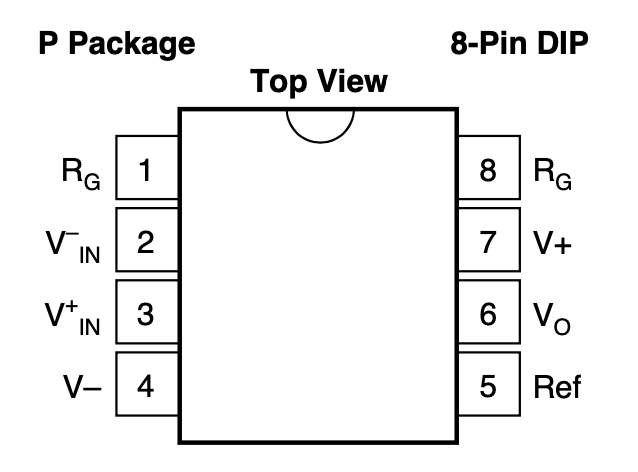
\includegraphics[width=0.5\textwidth]{../lessons/image/03/4.png}
\caption{\label{fig:3_4} Pin INA114AP.}
\end{figure}





\end{document}
